\documentclass[twoside]{article}

\usepackage{lipsum}
\usepackage[sc]{mathpazo}
\usepackage[T1]{fontenc}
\linespread{1.05}
\usepackage{graphicx}
\usepackage{microtype}
\usepackage[hmarginratio=1:1,top=32mm,columnsep=20pt]{geometry}
\usepackage{multicol}
\usepackage[hang, small,labelfont=bf,up,textfont=it,up]{caption}
\usepackage{booktabs}
\usepackage{float}
\usepackage{hyperref}
%\hypersetup{colorlinks=true}
\usepackage{lettrine}
\usepackage{paralist}
\usepackage{titlesec}
\titleformat{\section}[block]{\large\scshape\centering}{\thesection.}{1em}{}
\titleformat{\subsection}[block]{\large}{\thesubsection.}{1em}{}
\usepackage[nonumberlist]{glossaries}
\makeglossaries

% float-less figure for a multi-column environment
\newenvironment{flfigure}
  {\par\addvspace{\baselineskip}\begin{minipage}{\linewidth}
   \captionsetup{type=figure}}
  {\end{minipage}\par\addvspace{\baselineskip}}

\usepackage[backend=bibtex,style=numeric-comp]{biblatex}
\bibliography{index}

\title{\fontsize{14pt}{10pt}\selectfont\textbf{A New User Interaction Concept for Personal Information Management Systems}}
\author{
\large
\textsc{Vincent Wochnik}\\[2mm]
\normalsize Fontys University of Applied Sciences, Venlo \\
\normalsize \href{mailto:v.wochnik@student.fontys.nl}{v.wochnik@student.fontys.nl}
\vspace{-5mm}
}
\date{}

\begin{document}

\newglossaryentry{pims}{name=PIMS, description={Personal Information Management System}}

\maketitle
\begin{multicols}{2}
\section*{Abstract}

\noindent Conventional personal information management systems such as diaries, to-do lists and analog notebooks are rather inconvenient for the management of information since information that is once written down cannot easily be combined with other information or moved to a different place. This newly proposed system treats data which can be text, speech or images as atoms which can then be connected with each other. This way, it becomes very easy to manage information once in the system.

This is where smartwatches come into play: A smartwatch is a terrible device for actually managing information but is excellent for the input of such. Information that has been entered in the system can then be managend using traditional devices such as smartphones or personal computers.

\section{Introduction}

Kind of research: Explanatory empirical research

Research Topic: Personal Information Management Systems

Research Objective: Establish a relationship between the currently available personal information management systems such as to-do lists as well as notebooks and a newly proposed relational way of storing information and consolidate the claim that the newly proposed model is more effective.

Research Question and Subquestions

Is a relational approach to personal information management systems more efficient?
Do people prefer the current way of information management?
Do people accept the newly proposed model?

\section{Current Approaches}

Many approaches that aid in the visual representation and interaction with
unstructured data exist in the digital and analog world alike. A good example
thereof is the classical mind map which allows the establishment of connections
between unstructured information and thereby aiding in the emergence of a
structure.

Further approaches include the categorizing of information, visually
represented as folders or labels, establishing a timeline and attaching
information to various points in time as well as placing information inside a
coordinate system which is an excellent choice for prioritizing information
based on multiple criteria. Approaches using the coordinate system include
the \textit{importance-urgency matrix} or the \textit{growth-share matrix}.

However, there currently exists no viable solution allowing multiple approaches
to be applied to the same information in a way that allows ... in an every-day
context by the general user.

For example, it is currently not possible to connect various information in a
mind map and placing the same information in a coordinate system in such a way
that the visual representation can be interactively switched from the mind map
to the coordinate system.

To substantiate the example, let's imagine a mind map containing various goals
of an individual to provide a basic overview. Now, it would be handy to also
place the same goals in a coordinate system, say an \textit{urgency-importance
matrix}. If time constraints are given, another useful visual representation is
the timeline where the goals can be attached to specific points in time. This
is all possible with already existing systems. However, it is currently not
possible to interactively switch between the visual representations esily. This
is only made possible if the same information is placed within multiple models
at the same time and a system allows interactive switching of the model.

\section{Criteria of Acceptable Solutions}

The main criterion rendering a proposal acceptable is the remedy of the problem
outlined in the introduction of this article. Therefore, a proposed solution
must process information relationally instead of sequentially. The user must be
able to create relationships between bits of information easily and be able to
work with the information as in finding and retrieving information as well as
reorganizing existing information by changing relations without changing the
bits of information itself.

\iffalse
Relations -< verknüpfung (wort) unverständlich
\fi

Furthermore, a proposed solution should be relatively easy to use in comparison
to traditional \glspl{pims}. Therefore, the learning curve must not be too
steep and the user should become accustomed in relatively little amount of time.

\iffalse
Beispiel für diesen Use-Case
\fi

\section{Proposed Solution}

This proposed solution as an improved user interaction concept allows for a very
flexible and interactive \gls{pims} allowing the user
The proposal: An atomic data management system utilizing a smartwatch to take advantage of faster and more instantaneous data input.
The here proposed solution features a \gls{pims} supporting relationships
between bits of information. Since the proposed solution does not store
information sequentially but relationally, the reorganization of existing
information is possible without changing the information itself.

% deals with chunks of data

\subsection{Unstructured Data}

Various types of unstructured data can be seen in figure \ref{fig:unstructdata}
but unstructured data doesn't oppose any restrictions upon the user of the
\gls{pims} or what the implementation of such system itself. Basic
implementations can stick to text and graphical data. However, as the system
grows so do the needs of the user.

\begin{flfigure}
  \centering
    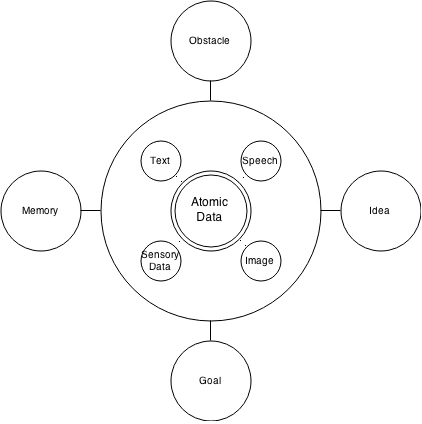
\includegraphics[width=0.9\linewidth]{00_resources/atomic_data.png}
    \caption{Unstructured data}
  \label{fig:unstructdata}
\end{flfigure}

Chunks of unstructured data can then be connected to other chunks by the user of
the system. The finer the chunks are, the more flexibility does the user have in
creating connections between chunks. A letter, for instance, can be inserted
into the system as one chunk of data which does not allow any connections within
the letter itself. However, the letter could also be inserted as multiple chunks
allowing the user to connect pieces of the letter to itself or other
information within the \gls{pims}.

\subsection{Data Sources}

In principle, any platform that implements a \gls{pims} that adheres to this
proposal can be a data source. However, this system is not meant to be
restricted to a particular platform but more so be a hub where any platform the
user chooses is supported in such a way that data can be inserted by the user.
Figure \ref{fig:datasources} shows a diagram of possible data sources across
multiple platforms.

\begin{flfigure}
  \centering
    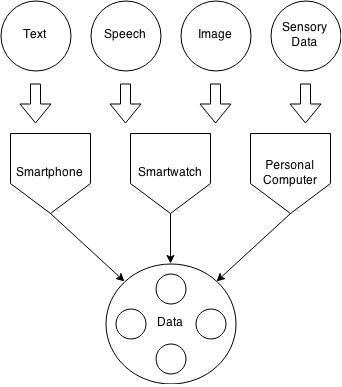
\includegraphics[width=0.9\linewidth]{00_resources/input_methods.png}
    \caption{Variety of data sources}
  \label{fig:datasources}
\end{flfigure}

\subsection{Organization of Data}

The organization of unstructured data is on a par with the available
visualizations thereof. That means that a \gls{pims} implementing all presented
visualizations allows the organization of unstructured data by any of those
visualizations or a combination thereof.

For instance, a system that supports connections between unstructured data and
a coordinate system must allow the user to connect chunks of unstructured data
with each other and simultaneously place these same chunks on a coordinate system.
A system need not support all visualizations presented in this paper or can
implement further visualizations not presented here.

Previously inserted atomic bits of data can be organized using a variety of models which are not all specified in this document. The more obvious ones are folders and labels as well as relationships between atomic data which can then be visualized as maps and radial relationship diagrams.

\subsection{Connections of Data}

Chunks of unstructured data can be connected to other chunks as shown in figure
\ref{fig:visualconnections}. The visualization can resemble a two-dimensional
map showing all chunks of data including its connections or can lean toward a
radial graph where the user can move through the connections by changing the
chunk in the center.

\begin{flfigure}
  \centering
    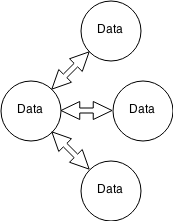
\includegraphics[width=0.5\linewidth]{00_resources/data_connections.png}
    \caption{Visualized relationships of unstructured data}
  \label{fig:visualconnections}
\end{flfigure}

\subsubsection{Labels}

Figure \ref{fig:visuallabels} shows the organization of chunks of data by
folders, here called labels. The visual representation looks quite similar to
the figure but can take other forms.

\begin{flfigure}
  \centering
    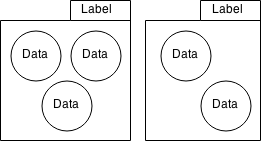
\includegraphics[width=0.5\linewidth]{00_resources/data_labels.png}
    \caption{Visualized labels of unstructured data}
  \label{fig:visuallabels}
\end{flfigure}

\subsubsection{Timeline}

\begin{flfigure}
  \centering
    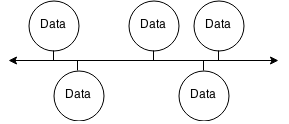
\includegraphics[width=0.5\linewidth]{00_resources/data_timeline.png}
    \caption{Visual timeline of unstructured data}
  \label{fig:visualtimeline}
\end{flfigure}

Data atoms can be ordered by time either manually specified or by the creation time of the data atom itself.

\subsubsection{Matrix}

\begin{flfigure}
  \centering
    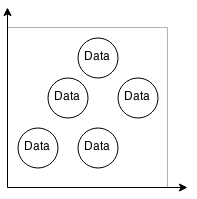
\includegraphics[width=0.5\linewidth]{00_resources/data_coord_system.png}
    \caption{Visual two-dimensional coordinate system of unstructured data}
  \label{fig:visualcoordsys}
\end{flfigure}

As seen in figure \ref{fig:visualcoordsys}, ...
Data atoms can be part of a two-dimensional matrix which can then be visualized.

\section{Conclusion}

blabla


% figures mit textverweis ! jede figure und caption

\printbibliography
\glsaddall
\printglossaries
\end{multicols}
\end{document}
